%%% Laboratory	 Notes
%%% Template by Mikhail Klassen, April 2013
%%% Contributions from Sarah Mount, May 2014
\documentclass[a4paper]{tufte-handout}

\newcommand{\workingDate}{\textsc{May $|$ 2014}}
\newcommand{\userName}{Felix Engstr\"o}
\newcommand{\institution}{KTH}

\usepackage{lab_notes}

\usepackage{hyperref}
\hypersetup{
    pdffitwindow=false,            % window fit to page
    pdfstartview={Fit},            % fits width of page to window
    pdftitle={Projekt lab notes 2016},     % document title
    pdfauthor={Felix Engstr\"om},         % author name
    pdfsubject={},                 % document topic(s)
    pdfnewwindow=true,             % links in new window
    colorlinks=true,               % coloured links, not boxed
    linkcolor=DarkScarletRed,      % colour of internal links
    citecolor=DarkChameleon,       % colour of links to bibliography
    filecolor=DarkPlum,            % colour of file links
    urlcolor=DarkSkyBlue           % colour of external links
}


\title{Projekt lab notes}
\date{2016}

\begin{document}
\maketitle

%%%%%%%%%%%%%%%%%%%%%%%%%%%%%%%%%%%%%%%%%%%%%%%%%%%%%%%%

\begin{projects}
	\begin{description}
		\item Things we plan to do 
	\end{description}
\end{projects}

%%%%%%%%%%%%%%%%%%%%%%%%%%%%%%%%%%%%%%%%%%%%%%%%%%%%%%%%
\newday{19 december 2016}

We have to day decided to try two approaches to the classification problem.
One: we use the states given in the training data to create two markow models,
one for the positive data and one for the negative data. We the use this model
to calculate the probability of the sequence we want to classify, if it is more
likely with the positive model, we classify it as positive, else it is
negative. Two: we are also going to try to train a neural network for the
classification problem. We are going to do this using an RNN(recurrent neural
network) with LSTM(long short-term memory) units. In the first step we are
going to disregard the data we have regarding the underlying statets and only
look at the binary classification problem. In a later stage we migth try to
train an ANN with the hidenstate data as target.


\begin{figure}
    \begin{center}
      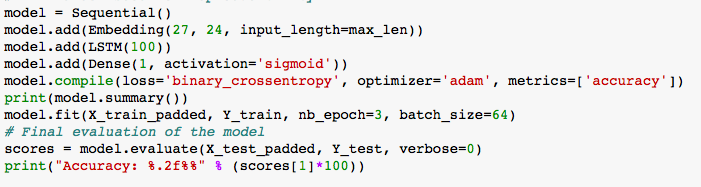
\includegraphics[width=0.8\textwidth]{pics/code_run_1.png}
    \end{center}
    \caption{Code for the first run.}
\end{figure}

This model was trained without dropout and with an embedding layer that was probably unneccesary.

\begin{figure}
    \begin{center}
      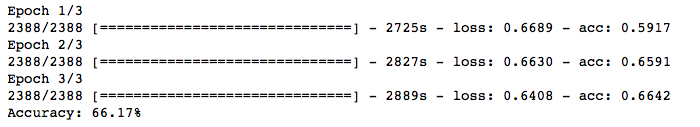
\includegraphics[width=0.8\textwidth]{pics/first_run.png}
    \end{center}
    \caption{Stats from the first run}
\end{figure}



\hrulefill

%%%%%%%%%%%%%%%%%%%%%%%%%%%%%%%%%%%%%%%%%%%%%%%%%%%%%%%%
\bibliographystyle{plain}
\bibliography{lab_notes}

\end{document}
